\section{Semana 07}

\lecture{7}{02 Outubro 2023}{Interface Gráfica}

Aplicações desktop e aplicações web são dois tipos distintos de softwares que se diferenciam principalmente pelo modo como são acessadas e executadas.

\textbf{Aplicação Desktop}
\begin{itemize}
    \item Execução Local: Roda diretamente no sistema operacional do computador do usuário.
    \item Acesso Offline: Pode ser usada sem a necessidade de uma conexão com a internet.
    \item Recursos do Sistema: Tem acesso direto aos recursos do sistema operacional e hardware.
    \item Instalação: Normalmente requer instalação e, por vezes, configuração no computador do usuário.
    \item Interface Gráfica: Usa os widgets e elementos de interface gráfica do sistema operacional.
    \item Atualizações: Os usuários geralmente precisam atualizar o software manualmente ou através de um sistema de atualização embutido.
    \item Exemplo de Tecnologia: Tkinter, PyQt para Python.
\end{itemize}

\textbf{Aplicação Web}
\begin{itemize}
    \item Execução Remota: Roda em um servidor web e é acessada por meio de um navegador de internet.
    \item Acesso Online: Geralmente, necessita de uma conexão com a internet para ser utilizada (a menos que seja projetada para funcionar offline).
    \item Recursos Limitados: As operações no lado do cliente têm acesso limitado aos recursos do sistema do usuário devido às restrições de segurança do navegador.
    \item Sem Instalação: Não requer instalação no computador do usuário, apenas um navegador web.
    \item Interface Gráfica: Usa tecnologias web (HTML, CSS, JavaScript) para a interface, sendo independente do sistema operacional.
    \item Atualizações: Atualizações são feitas no servidor, sem necessidade de intervenção do usuário para atualizar a aplicação.
    \item Exemplo de Tecnologia: Flask, Django, Tornado para Python.
\end{itemize}

\subsection{Aplicação Web}

No código, foi adicionado um novo endpoint e um método para renderizar uma página HTML simples:

\begin{verbatim}
# Importando módulo para renderização de templates do Tornado
from tornado.web import RequestHandler, Application, url

# ...

class SparqlQueryHandler(RequestHandler):
    def get(self):
        # Renderizando o template HTML no acesso GET
        self.render("sparql_query.html")
    
    def post(self):
        # Obtendo a consulta SPARQL do formulário
        sparql_query = self.get_body_argument("sparql_query")
        
        # Executando a consulta
        results = g.query(sparql_query)
        
        # Enviando os resultados para serem exibidos no HTML
        self.render("sparql_query.html", results=results.serialize(format="json"))

class SPARQLServer(Application):
    def __init__(self):
        handlers = [
            ("/sparql", SPARQLHandler),
            ("/query", SparqlQueryHandler)  # Adicionando novo endpoint
        ]
        super(SPARQLServer, self).__init__(handlers)
\end{verbatim}

E foi criado um arquivo sparql\_query.html com um formulário HTML básico para input da consulta SPARQL e exibição dos resultados.

\begin{verbatim}
<!DOCTYPE html>
<html lang="en">
<head>
    <meta charset="UTF-8">
    <meta name="viewport" content="width=device-width, initial-scale=1.0">
    <title>SPARQL Query Interface</title>
</head>
<body>
    <h1>Execute SPARQL Query</h1>
    <form method="post" action="/query">
        <label for="sparql_query">SPARQL Query:</label><br>
        <textarea name="sparql_query" id="sparql_query" rows="4" cols="50"></textarea><br>
        <input type="submit" value="Execute Query">
    </form>
    
    
    <h2>Results:</h2>
    <pre>{{ results }}</pre>
    
</body>
</html>
\end{verbatim}

\subsection{Exemplo}

Para o exemplo, foi colocado no SPARQL Query o seguinte comando: "SELECT * WHERE { ?s ?p ?o . }"

\begin{figure}[htpb]
    \centering
    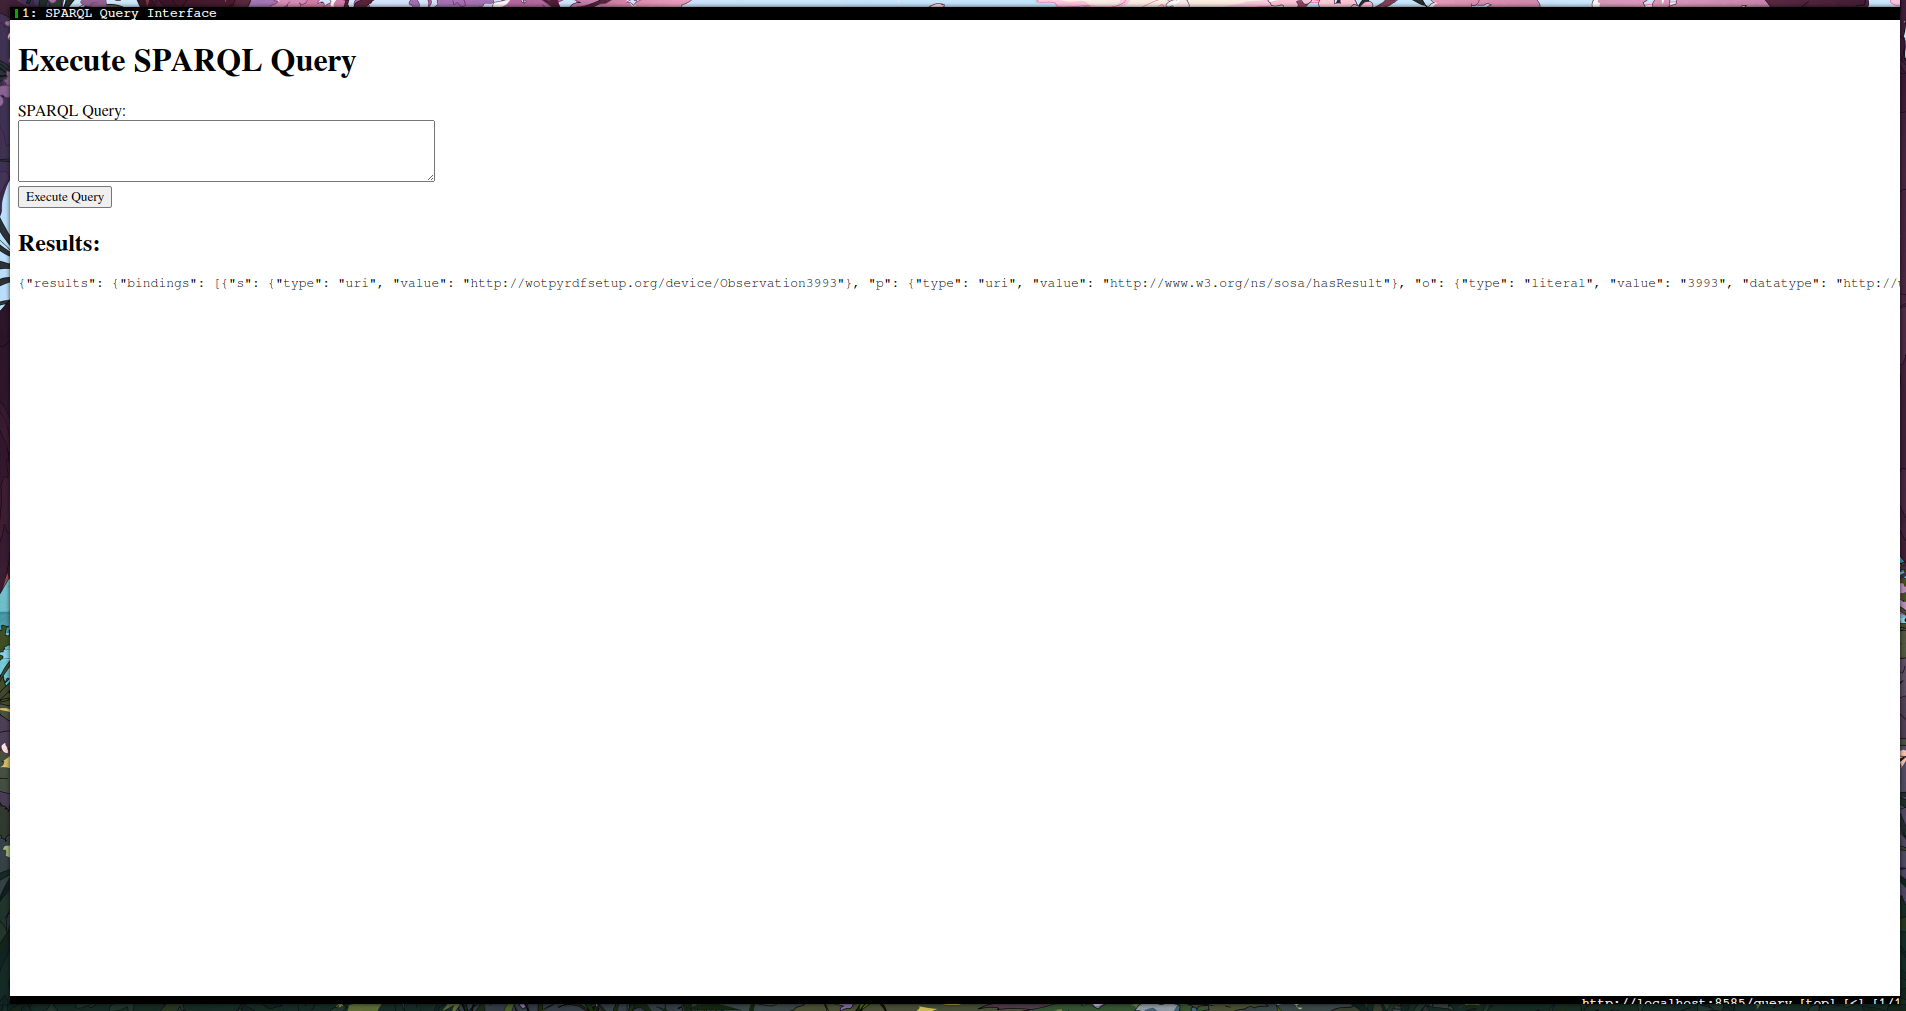
\includegraphics[scale=0.3]{figures/example1.png}
    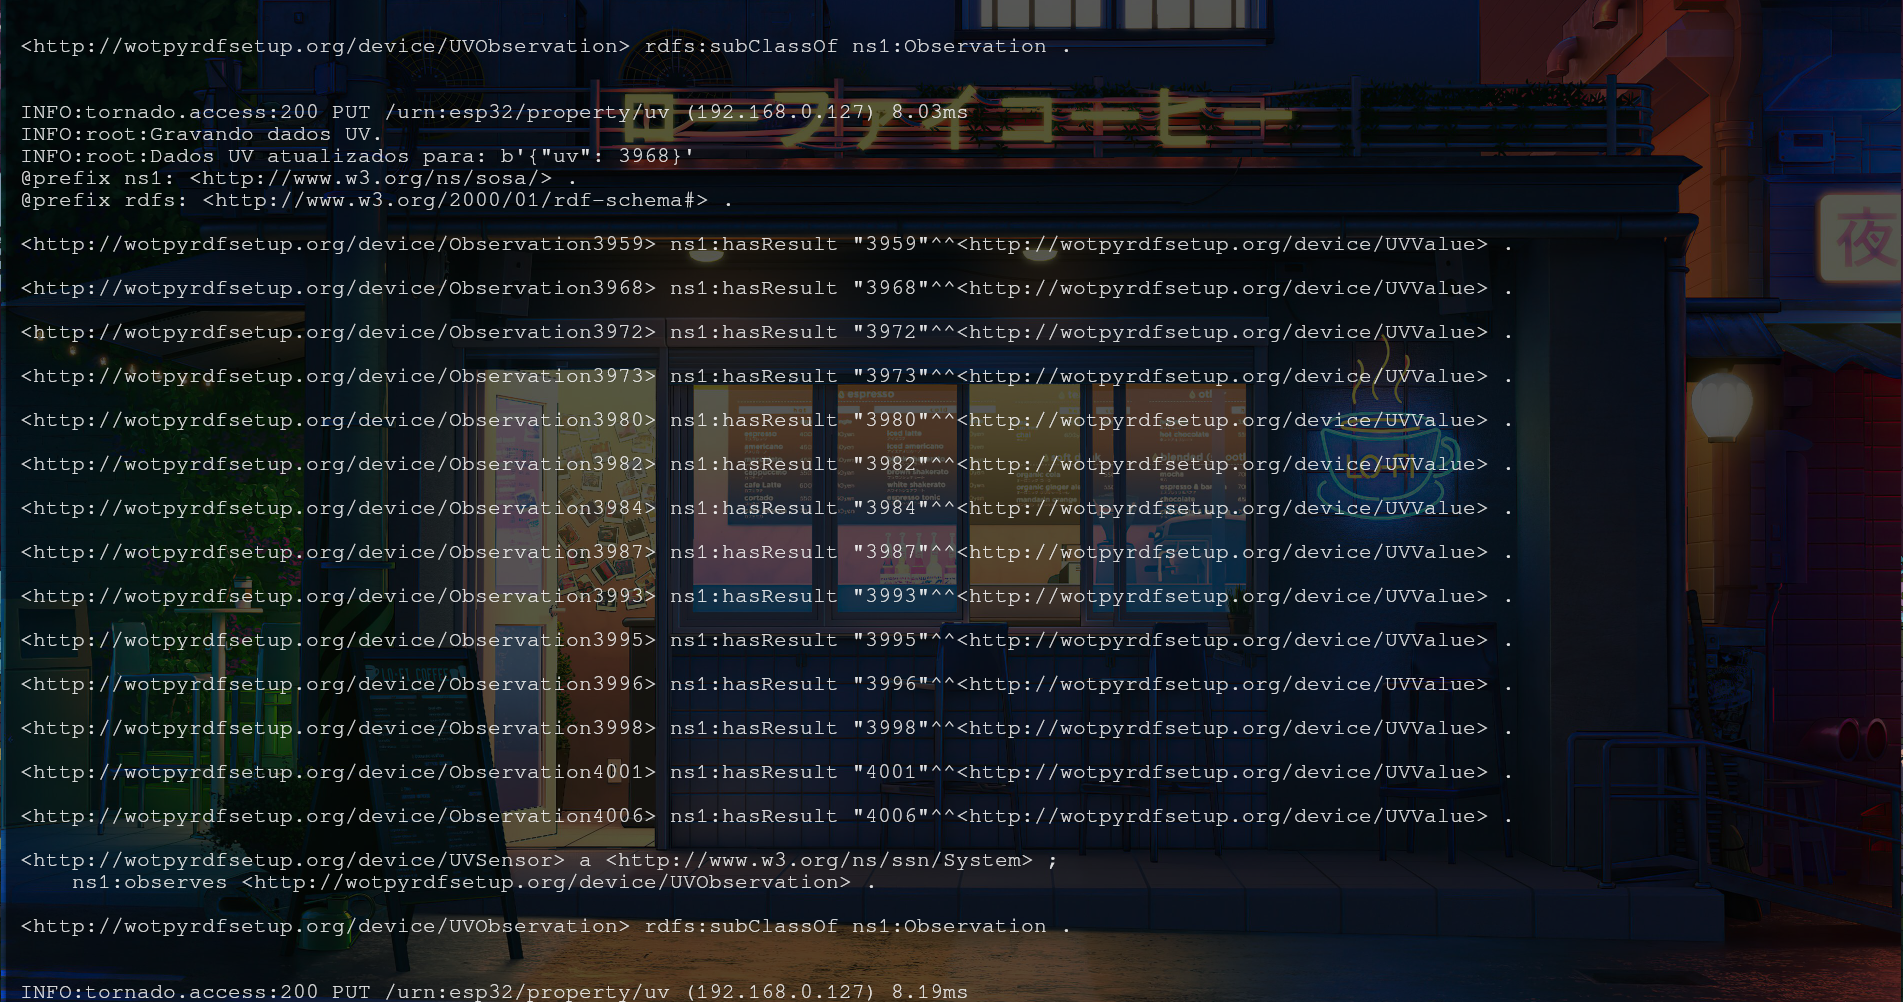
\includegraphics[scale=0.3]{figures/example2.png}
\end{figure}


